\documentclass[11pt,a4paper]{article}

\usepackage[utf8]{inputenc}
\usepackage[margin=0.75in, paperwidth=8.5in, paperheight=11in]{geometry}
\usepackage{amsfonts, amsmath, amssymb}
\usepackage[none]{hyphenat}
\usepackage{fancyhdr} %Allows us to create custom header and footer
\usepackage{float}
\usepackage{lmodern}
\usepackage[T1]{fontenc}
\usepackage{gensymb}
\usepackage{siunitx}
%\usepackage[section]{placeins}
\usepackage[nottoc, notlot, notlof]{tocbibind} %Buttify this LOL

%% For Background Setup i.e, WaterMark %%
\usepackage{tikz}
\usetikzlibrary{calc}

%% For Underlining %%
\usepackage{ulem}
\renewcommand{\ULdepth}{1.8pt}

%% For Inserting Figures %%
\usepackage{graphicx}
\usepackage{lipsum}
\usepackage[export]{adjustbox}
\usepackage{wrapfig} %It takes two parameters that are passed inside braces: the alignement that can be l, r, c, i or o; this letters stand for left, right, centre, inner and outer (the last two intended for two-sided documents). The second parameter is the width of the figure
\usepackage{caption}
\usepackage{subcaption}
%\graphicspath{{../Lab-2/Screenshots/}{../Lab-3/}{../Lab-4/}{../Lab-5/}{../Lab-6/}{../Lab-7/}{../Lab-8/}{../Lab-9/}{../Lab-10/}{../Lab-11/}}

\pagestyle{fancy}
\fancyhead{} %This will clear the default header value
\fancyfoot{}
\fancyhead[L]{\slshape \MakeUppercase{IoT Room Automation Report}}
\fancyhead[R]{\slshape Dharan Teja}
\fancyfoot[c]{\thepage}

\renewcommand{\baselinestretch}{1.5} %This will effect the line spacing between two lines

\begin{document}

%----------------------------------------------------------------------------------------
%	TITLE PAGE
%----------------------------------------------------------------------------------------

\begin{titlepage} %Suppresses displaying the page number on the title page and the subsequent page counts as page 1

\newcommand{\HRule}{\rule{\linewidth}{0.5mm}} %Defines a new command for horizontal lines, change thickness here

%%Page Border-Line Setup--
\begin{tikzpicture}[remember picture,overlay]
   \draw[line width = 2pt] ($(current page.north west) + (0.5in,-0.5in)$)  rectangle ($(current page.south east) +  (-0.5in,0.5in)$);
\end{tikzpicture}

\begin{center}
\vspace*{3.3cm}
\textsc{\LARGE{Project Report}}\\
\vspace*{1cm}

\HRule\\[0.4cm]	
\Huge{\bfseries{IoT ROOM AUTOMATION}}\\
\Huge{\bfseries{using PIC16F887 and NodeMCU}}\\[0.4cm]
\HRule\\[1.5cm]

\begin{minipage}{0.4\textwidth}
		\begin{flushleft}
			\large
			\textit{Created by}\\
			\textsc{Dharan Teja Vipparla}\\ % Your name
		\end{flushleft}
	\end{minipage}
	~
	\begin{minipage}{0.4\textwidth}
		\begin{flushright}
			\large
			\textit{Reviewed by}\\
			\textsc{Amit} Sir,\\ % Supervisor's name
			CTO of \textsc{Pragyatmika}\\
		\end{flushright}
	\end{minipage}

\vfill\vfill\vfill %Automatically adjust the date 3/4 down the remaining page

{\large{\today}}
\vfill	%Push the date up 1/4 of the remaining page

\end{center}

\end{titlepage}

%----------------------------------------------------------------------------------------

%----------------------------------------------------------------------------------------
%	ACKNOWLEDGEMENT
%----------------------------------------------------------------------------------------

\begin{center}

\Large{\bfseries{ACKNOWLEDGMENT}}\\
\vspace*{2cm}

\end{center}
\parindent 0ex %Paragraphs will not be indentend automatically.. everything is flushed left

I would like to express my special thanks of gratitude to "\uline{Amit Sir}", CTO of Pragyatmika The Power of Intelligence for his guidance and also for his constant support in completing this project of "Room Automation over IoT", which also helped me in doing a lot of research, and I came to know about many different things from basic electronic components and tools to several latest industrial innovations and technologies.\\ 

Through this project and his guidance, I've build a strong base over "C" Language and I am able to gain experience in "IoT \& Embedded systems" design along with preemptive, multitasking real-time operating systems. And I became very familiar with using Software platforms like \textit{MPLAB X IDE, Arduino IDE} and Simulation platforms like \textit{Proteus}, and Cloud Platforms like \textit{ThingSpeak, Adafruit, IFTTT, Blynk} for IoT \& Cloud Communication, and Hardware tools like \textit{LCD, Seven segment displays, ADC Converters, Sensors, RTC Chips, Relays, Micro-Controllers} and several other hardware modules. And I also gained adequate knowledge of reading schematics and data sheets for components.\\

Therefore once again I am expressing my sincere gratitude to Amit Sir and my Parents for helping and constantly supporting me in doing this innovative project, giving me a parcel of data about the future innovation and the utilization of home automation framework in our everyday life.\\

\vfill
Thank you.
\vfill\vfill\vfill

\thispagestyle{empty} %This will remove Header and Footer of this page
\clearpage %Clears the Page Number of this page 
\newpage

%----------------------------------------------------------------------------------------

%----------------------------------------------------------------------------------------
%	TABLE OF CONTENTS
%----------------------------------------------------------------------------------------

\begin{center}

\vspace*{1cm}
\Large{\bfseries{ABSTRACT}}\\
\vspace*{1cm}

\end{center}
\parindent 0ex %Paragraphs will not be indentend automatically.. everything is flushed left

Home automation develops the lifestyle by automating the appliances. It is a technique or a system of controlling a process by electronic devices with reducing human involvement to a minimum.  It saves energy as well as time. This project aims to achieving the design and model implementation of the home automation system using sensors readings and applying the Internet of Things
(IoT) and Bluetooth technologies.\\

Home Automation using cloud network is a system that uses computers or mobile devices to control basic home functions and features automatically through the internet from anywhere around the world, an automated home is sometimes called a \uline{smart home}. Many electrical appliances like fan, light can be controlled using android operating system.\\

This systems mainly consist of a Smart-phone, Switch Buttons, and Micro-controllers. We use Smart phone to give orders to units that we wish to control locally or remotely and the Micro-controller is used as an appropriate interface to sensors and appliances of a home automation system and communicates with an android application through wireless technology. We use Switch buttons to switch between Bluetooth and WiFi mode for the communication. This system also consists of a extra feature which is the Digital Clock, which gives real time data to the micro-controller and can be operated with ease by the user to set time, date, day, month, etc., and is displayed in LCD. 

\thispagestyle{empty} %This will remove Header and Footer of this page
\clearpage %Clears the Page Number of this page 
\newpage

%----------------------------------------------------------------------------------------

%----------------------------------------------------------------------------------------
%	TABLE OF CONTENTS
%----------------------------------------------------------------------------------------

% Change the name of the ToC
\renewcommand\contentsname{\LARGE\textsc{CONTENTS}}

\tableofcontents
\thispagestyle{empty} %This will remove Header and Footer of this page
\clearpage %Table of contents will be on its own page 
%----------------------------------------------------------------------------------------

\setcounter{page}{1} %This will count page numbers from 1 from introduction page

%%Lets begin Theory!!
%----------------------------------------------------------------------------------------
%	EXPERIMENT-1
%----------------------------------------------------------------------------------------
\section{Introduction}

\parindent 0ex %Paragraphs will not be indentend automatically.. everything is flushed left
It is well known that the concept of smart home has focused the attention of researchers, lifestyle practitioners, and the consumers to be directed forward the usage of the recent technology. The use of smart devices in daily activities increases the quality of life and offers high productivity in turn. The concepts of modern smart home are referred to the home automation systems which are designed based on different technologies. The main purpose of home automation system is to save human effort, cost reduction, money, time and electricity, and have centralized control of appliances.\\

Hence in this project, I designed a home automation system which can be operated or controlled by any one with ease. This is secured, flexible and user friendly in terms of operation. It can also be operated by Bluetooth connectivity which provides the capability to control and monitor the home appliances and other household activities.\\ 

This system can count the number of people entered or exited the room with very few errors, and controls the settings of lights(Brightness, Dimming, Switching(ON/OFF)) as per the people present in particular room.\\

\subsection{IoT Technology:}
The inter-connectivity of virtually every object is now possible through the Internet, human social networks, and machine-to-machine communications.\\

IoT involves integrating smart objects, embedded devices with sensors and actuators connected to the Internet. These devices are intelligently interconnected thereby necessitating new forms of communication between things and people, and between things themselves(collect and exchange
data).When IoT is augmented with sensors and actuators, the technology becomes an instance of the more general class of cyber-physical systems, which also encompasses technologies such as smart grids, smart homes, intelligent transportation and smart cities.\\

The modern society brings varied information where safe, comfortable and convenient life has become the ideal for new technology end-users. For that, the IoT technology becomes a hot research topic
especially in becoming the main feature for the coming 5G communication technology.
\newpage

\subsection{Implementation Setup:}
The key hardware components that make up this room automation system are:

\begin{enumerate}
\item PIC16F887 Micro-controller Development Board
\item WiFi integrated ESP8266 SoC NodeMCU Board
\item Bluetooth (HC-05) module
\item IR and PIR Sensors 
\item Relay boards 
\item Electric Appliances (Bulbs as Prototypes)
\item 16x2 char LCD 
\item Real Time Clock chip (DS3231)
\item LEDs and Switches
\item Smart Phone
\end{enumerate}

\begin{figure}[!htbp]
  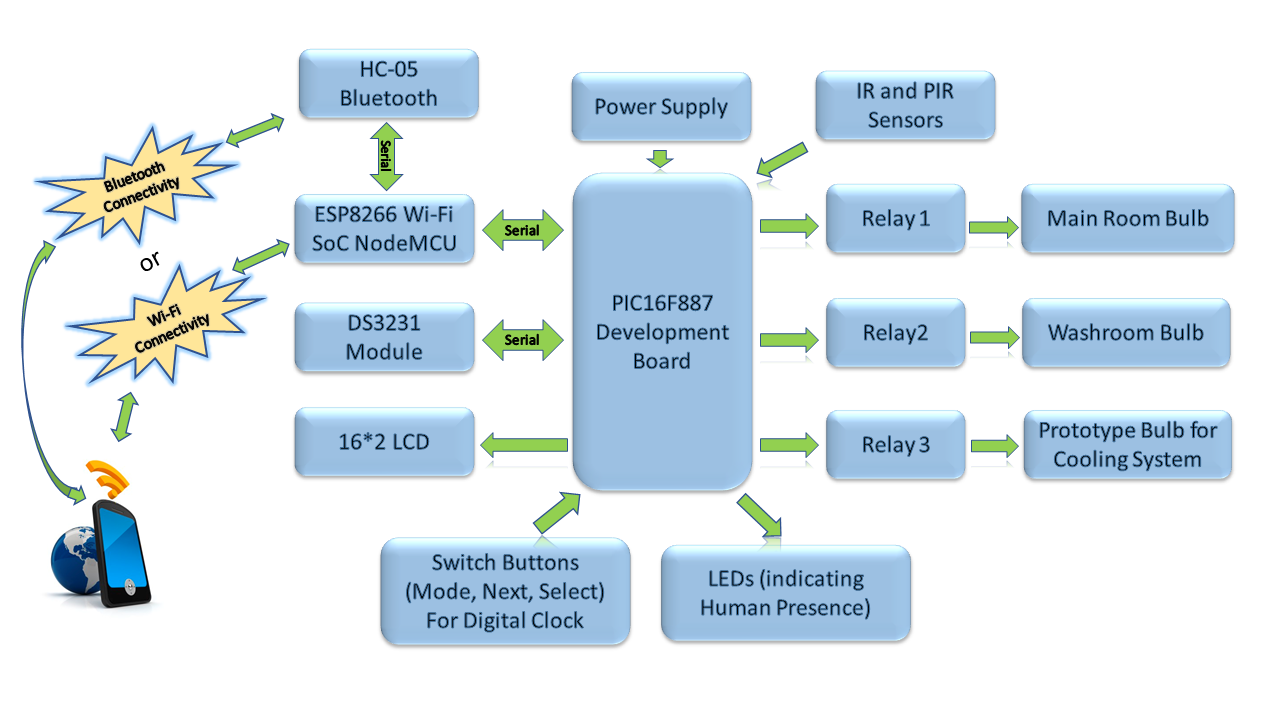
\includegraphics[width=\linewidth]{Block Representation.png}
  \caption{Block Representation of the System}
  \label{fig:Block Representation of the System}
\end{figure}

\newpage

In hardware implementation, we are using \textbf{PIC16F887} micro-controller as a main controller for sensors interfacing and is connected to other hardware components. I've used a \uline{PIC16F887 development board} manufactured by Microchip company. PIC16F887 does not have any wireless connection, that's why we are using a WiFi module for wireless communication. \textbf{ESP8266} WiFi integrated SoC NodeMCU board is
used for wireless communication between android mobile app and NodeMCU board. If a person uses \uline{Google Assistant} and give a voice command for controlling a certain electrical appliance, then  the NodeMCU board processes the received command using MQTT Protocol (used for sending and collecting data to the device cloud platform, Adafruit) and passes the control over to PIC16F887 board to control the electrical appliances.\\

Also \textbf{HC-05} Bluetooth module is used, which is connected to NodeMCU Board, so that we can control our appliances through the Bluetooth also, in a range anywhere between 1-10 meters. Similar to WiFi Communication method, NodeMCU processes the received command when user controls certain appliance using \textit{\uline{Bluetooth Controller App}} in Smart-Phone and passes the control over to the PIC16F887 board which will generate output based on the command received. One important thing to note is, when using Bluetooth connectivity for controlling appliances we can't use WiFi connectivity and vice-versa.\\ 

For electrical switches we use \textbf{Relay board} that is connected to PIC16F887. Here in our system, 3 relays are used to control AC bulbs. (For the Dimmable Bulbs(Washroom LED and Cooling System prototype), we must use TRIACS or Solid-State-Relays. But for the Demo purpose, I've used only one mechanical relay in this project which will control the Main-room's Light Bulb, and for controlling Washroom's Bulb and Cooling System, I've grouped some LEDs and used transistors to drive them from PWM output of PIC16F887 Micro-Controller)\\

To get the real time data, \textbf{DS3231 RTC} (Real-Time-Clock) module is used. With the help of this module, I've implemented a Digital Clock through which we can set the time (even in AM and PM modes) and calender using switch buttons.\\

\textbf{IR} and \textbf{PIR} sensors connected to PIC16F887 board are used for human detection and having control over the electrical appliances switching depending upon whether there is a person in the room or not. If a human is present in room, then a small LED attached to the outer side of the door will be turned on indicating the human presence in the room.\\

\newpage

\section{Hardware Modules:}
\subsection{PIC16f887 Development Board:}

\begin{figure}[!htbp]
  \begin{subfigure}[b]{0.5\textwidth}
    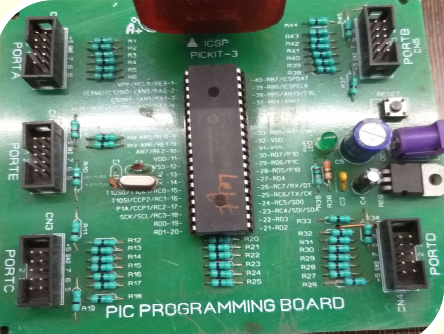
\includegraphics[width=\textwidth]{PIC16F887 Dev Board.png}
    \caption{PIC16F887 Development Board}
    \label{fig:PIC16F887 Development Board}
  \end{subfigure}
  \hfill
  \begin{subfigure}[b]{0.5\textwidth}
    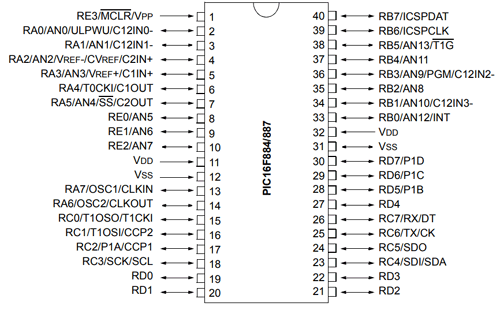
\includegraphics[width=\textwidth, height=6.7cm]{PIC16F887-Pinout.png}
    \caption{PIC16F887 Pin-out}
    \label{fig:PIC16F887 Pin-out}
  \end{subfigure}
  \caption{PIC16F887 Board}
\end{figure}

PIC16F887 is a 8-bit 40-pin IC. It has \uline{35 I/O Pins, 1 extra Input Pin and 4 Power pins}.  It has \textit{14 Channel 10-bit ADC} making it suitable for applications which require more ADC inputs. The IC also has \textit{2 Comparators}, \textit{2 Timers} (8-bit and 16-bit) and supports \textit{SPI, I2C and UART communication protocols}. It has a \uline{\textit{RAM} of 368 Bytes} and \uline{\textit{EEPROM} of 256 Bytes}.

It can operate at a speed of upto \textit{20MHz with External Oscillator} and also has precision \textit{Internal Oscillator tunable between 8MHz to 32kHz}.

The IC also supports safety features like \textit{Power-on Reset (POR), Brown-out Reset (BOR), Low Current Watchdog Timer (WDT), etc.}, making it suitable for critical tasks and industrial applications.\\

PIC16F887 development board is integrated with many active and passive electrical components like \textit{Resistances, Capacitors, Switches, LEDs, Voltage Regulator, Oscillator, etc}.
In order to program the PIC16F887 we use \uline{\textit{MPLABX v3.35 IDE}} (Integrated Development Environment), where the programming takes place, and \uline{\textit{XC8} compiler}, where our program gets converted into MCU readable form called HEX files.\\

To dump or upload our code into PIC, we use a device called \uline{PICkit-3}. The PICkit-3 programmer/debugger is a simple, low-cost in-circuit debugger that is controlled by a PC running MPLAB IDE (v8.20 or greater) software on a Windows platform. The PICkit 3 programmer/debugger is an integral part of the development engineer's tool suite.
\newpage

\subsection{NodeMCU Board:}

\begin{figure}[!htbp]
  \begin{subfigure}[b]{0.5\textwidth}
    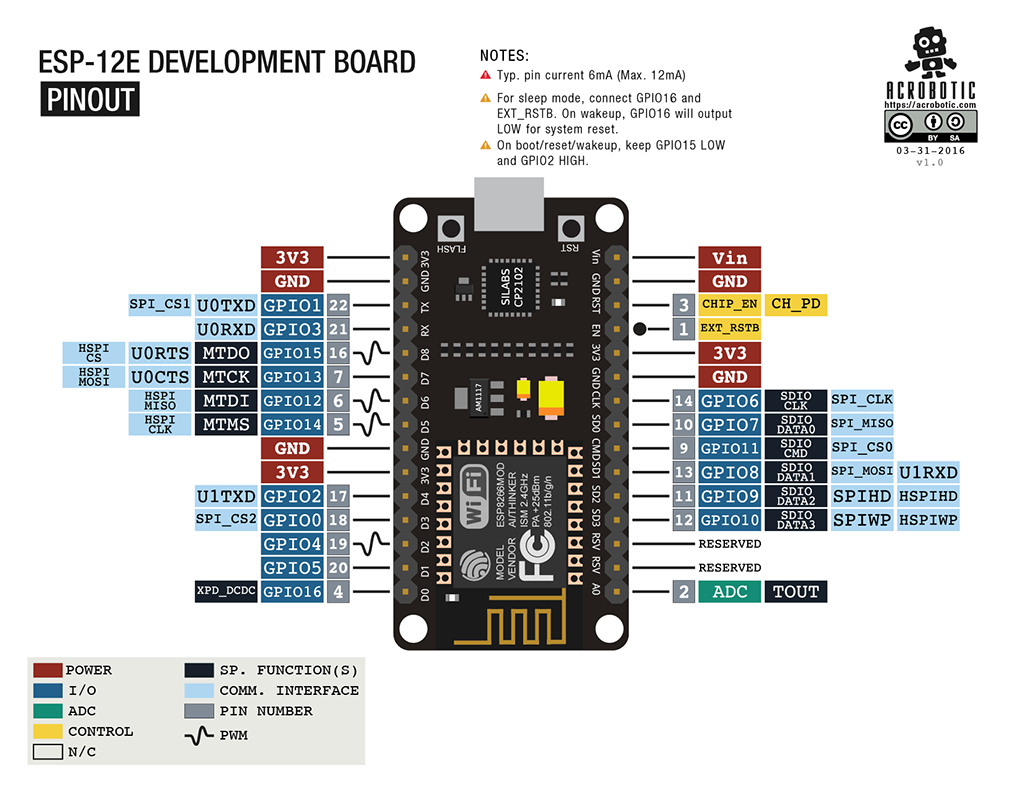
\includegraphics[width=\textwidth]{ESP-12E Development Board Pin Out.png}
    \caption{ESP-12E Development Board Pin Out}
    \label{fig:ESP-12E Development Board Pin Out}
  \end{subfigure}
  \hfill
  \begin{subfigure}[b]{0.5\textwidth}
    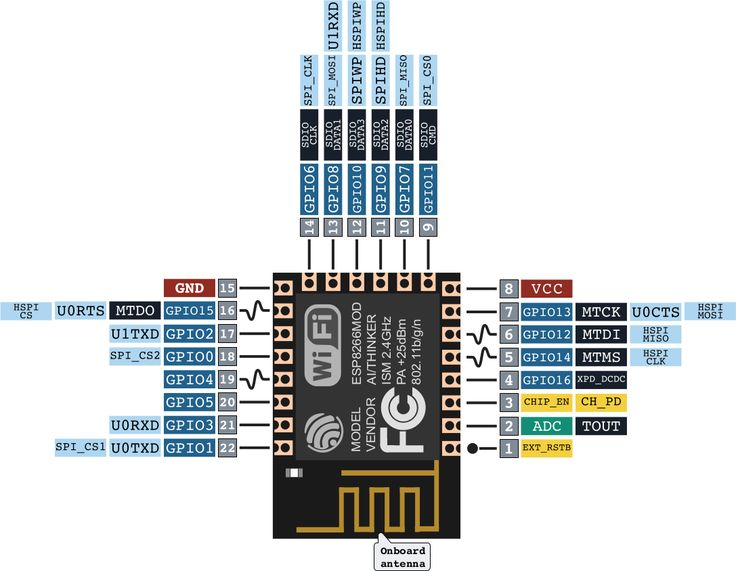
\includegraphics[width=\textwidth, height=6.7cm]{ESP-12E Pin Out.jpg}
    \caption{ESP-12E Pin Out}
    \label{fig:ESP-12E Pin Out}
  \end{subfigure}
  \caption{NodeMCU}
\end{figure}

NodeMCU Development Kit/board consist of ESP8266 wifi enabled chip. The ESP8266 is a low-cost Wi-Fi chip developed by Espressif Systems with \textit{TCP/IP} protocol. NodeMCU Dev Kit has Arduino like Analog (i.e. A0) and Digital (D0-D8) pins on its board.\\

In this project, NodeMCU is used mainly for \textit{IoT} Application and Bluetooth Communication. After setting up ESP8266 with Node-MCU firmware in \textit{Arduino IDE}, it is programmed using software serial port configuration method for PIC16F887-ESP8266 Communication after implementing \textit{'USART Protocol'} in PIC16F887 for \uline{Master to Master Communication}.

\subsubsection{MQTT IoT Protocol:}

MQTT, \uline{Message Query Telemetry Transport} Protocol is used for ESP8266 device's \uline{Commissioning} (taking the device to the Network) and \uline{Provisioning} (Device uses WiFi facilities).

MQTT uses TCP/IP Protocol layer. It has three main components:

\begin{itemize}
\item \textbf{Subscriber -} Subscriber is a Receiver which requests the requiring data which is reposited in Cloud platform by subscribing to a particular "topic" in a cloud platform.

\item \textbf{Publisher -} Publisher is a Sender which collects and sends the data to subscriber by pushing a message to a "topic"  in the cloud platform.

\item \textbf{Broker -} Broker is a Cloud Platform (Adafruit, Thingspeak, etc), whose main task is Authorization (IP, Server address) of Publishers and Subscribers, and ensuring security. It ensures whether all the subscribers receiving messages from the topic they subscriber or not.
\end{itemize}

\subsubsection{Adafruit Device-Cloud Platform:}

Adafruit is a IoT Device Cloud based server deployment responsible for:

\begin{itemize}
\item User/Device Authentication
\item User-Device linking
\item Device control and interface management
\item Geo-location (where device is located)
\end{itemize}

\begin{figure}[!htbp]
	\centering
  	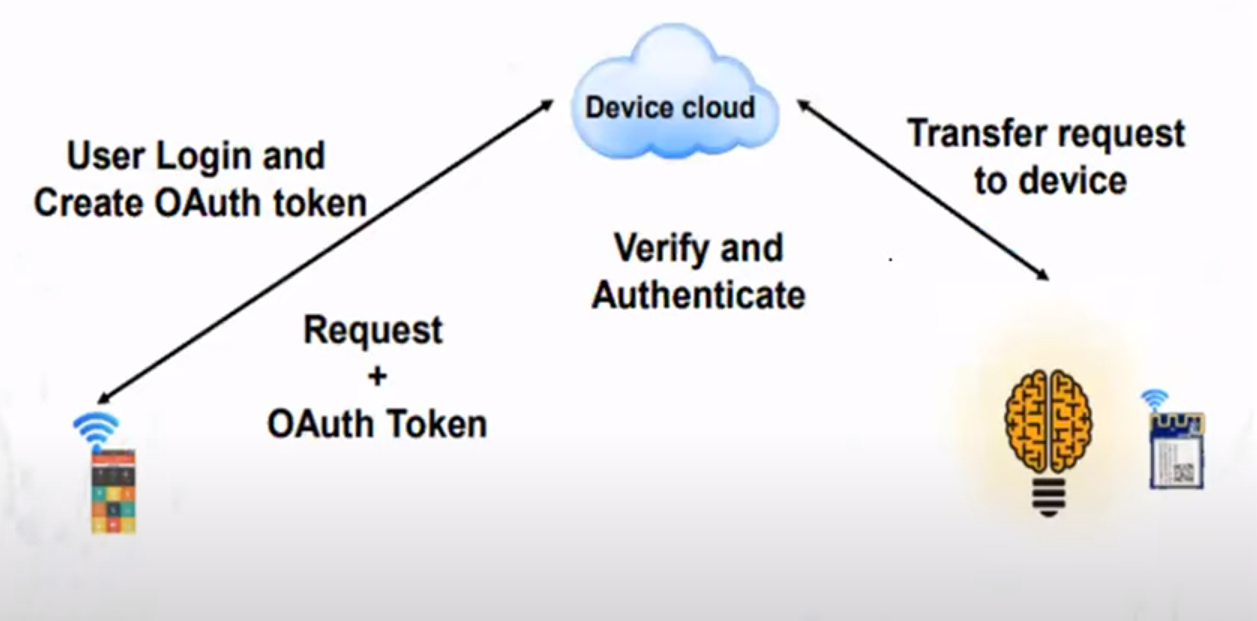
\includegraphics[width=0.9\linewidth]{User association.png} 
	\caption{User Association with the Device-Cloud}
	\label{fig:Adafruit-User Association}
\end{figure}

Steps involving user association with the Adafruit cloud platform include:

\begin{enumerate}
\item Firstly, Device(ESP8266) gets provisioned by Smart-phone.
\item Then Mobile sends the 'Authentication token' to the Device-Cloud for storing Device's data
\item Device-Cloud then verifies and sends the 'Authentication token' to the Device, if matches then Device gets stored in Device-Cloud. 
\end{enumerate}


MQTT Protocol is implemented in Arduino IDE for making ESP8266 device's connection to \textit{Adafruit} Cloud Platform and is made ensured that device stays connected to Cloud platform at all times.

\subsubsection{WiFi Communication with PIC16F887 Micro-Controller:}

After the successful connection with the Adafruit Device-Cloud, 

\begin{enumerate}
\item When the user sends a command through Google Assistant, then that information will be passed to Adafruit Cloud Platform after some Authentication process. Then the Device cloud passes it's status to the ESP8266 Micro-Controller.

\item Therefore, ensuring whether the status of the Device-Cloud(i.e, Adafruit) is receiving or not is the task of Espressif ESP8266 Micro-Controller.

\item And then it sends the received status or commands to PIC16F887 Micro-Controller.

\item In the end, PIC16F887 will take the actions on the electrical appliances based on the command received from ESP8266.    
\end{enumerate}

\subsection{HC-05 Bluetooth Module:}

\begin{wrapfigure}{R!htbp}{0.4\textwidth}	%Wrapping Text around a figure
\centering
\includegraphics[width=0.9\linewidth]{HC-05.jpg} 
\caption{HC-05 Bluetooth Module}
\label{fig:HC-05 Bluetooth Module}
\end{wrapfigure}

Since home automation systems are designed based on different technologies, here in this project, we can also use Bluetooth connectivity to control the electrical appliances wirelessly with ease. Bluetooth
technology is also low cost and secure.\\

This HC-05 Bluetooth module allows us to wirelessly transmit and receive data. The module that we’re using is based on the \uline{Bluetooth v2.0 protocol} and is having a \uline{range of 10 meters} operating at \uline{frequency of 2.4GHz} with a \uline{maximum data exchange rate of 2.1Mbps}.  Initially a password enabled method is used to pair the Bluetooth module with a mobile phone. After the \uline{password 1234} is given, the HC-05 module is paired with Android mobile phone.\\ 

The home appliances (based on this project) like lights, Cooling systems will turn ON and OFF when the user press a button in the \textit{Bluetooth Terminal App} in smart-phone. The command will be passed to the Bluetooth module and then transmitted to ESP8266, which will process the command and transimit the status to the PIC16F887 Micro-Controller via USART Communication.
\newpage

\subsection{IR Sensor Module:}

\begin{wrapfigure}{R!htbp}{0.4\textwidth}	%Wrapping Text around a figure
\centering
\includegraphics[width=0.9\linewidth]{IR Sensor.jpg} 
\caption{IR Sensor Module}
\label{fig:IR Sensor Module}
\end{wrapfigure}

IR technology is used in daily life and also in industries for different purposes. The main benefits of IR sensors are low power usage, their simple design \& their convenient features.\\

An infrared sensor is an electronic device, that emits infrared radiation in order to sense some aspects of the surroundings. It can measure the heat of an object as well as detects the motion. IR signals are not noticeable by the human eye, but can be detected by these sensors.\\

I have used \uline{four IR sensors} in this project, \uline{2 for Main door} and \uline{2 for Washroom Door}. One IR sensor is attached to outer part the door and the other one is attached to the inner part of the door.\\

\subsubsection{Control over Mainroom's and Washroom's Appliances:}
\begin{itemize}
\item For the control over \textit{Main room's electrical appliances}, with the help of these IR Sensors, I have programmed in such a way that whenever a person enters the room, the count will increase, and it decreases when people exit. If the Count is greater than 0, then it indicates a human is present in the room, hence he can control the appliances. If the count becomes 0, then it means no one is in room, Therefore all the electrical appliances gets turned OFF.

\item For the \textit{Washroom's Light}, \uline{PIR sensor} is used to turn ON the light after detecting human presence. In this case, only if the person exits the washroom (not while entering the room), IR sensors attached to the Washroom door are used to turn OFF the washroom light. Here, IR Sensors are not used for the purpose of counting the people, instead these are used to just turn OFF the Light which was turned ON by the PIR sensor after detection. In this case false detections are very minimal since three sensors are used for the control over washroom appliance.
\end{itemize}
\newpage

\subsubsection{Drawbacks of using IR Sensors:}
\begin{enumerate}
\item One major problem when using IR sensors for counting the number of people entered in the room is, sometimes these sensors can get \uline{tripped or detect falsely} (maybe because of ambient light, or it may have detected some other heat emitting objects/beings, or if a person just knocks on the door and leave without entering, etc). 

To solve this problem, I have used the concept of Timers, so that after the IR sensor detects a object, the \uline{detection case is considered only for 2 seconds}, after that it won't be considered. In programming terms, the \textit{flag} which is used to set HIGH when IR detects will be cleared after 2 seconds of time instead of leaving it in HIGH state forever. Refer Section 4.1

\item It is important to note that, we don't always get the correct Count result through these IR Sensors, since sometimes door can be left half open or slightly left open. Therefore, other methods like using \textit{Finger-Print Scanner} or usage of \textit{CC Cameras and Machine Learning} should be taken into consideration for the counting purpose. But I've considered it for the future scope of this project.
\end{enumerate} 

\subsection{PIR Sensor Module:}

\begin{wrapfigure}{R!htbp}{0.5\textwidth}	%Wrapping Text around a figure
\centering
\includegraphics[width=1.0\linewidth, height = 5cm]{PIR Sensor.jpg} 
\caption{PIR Sensor Module}
\label{fig:PIR Sensor Module}
\end{wrapfigure}

A Passive Infrared Sensor is an electronic sensor that measures infrared light radiating from objects. PIR sensor detects a human being moving around within approximately 10m from the sensor. These are fundamentally made of a Pyro-electric sensor, which can detect levels of infrared radiation. The image shows the pin out and circuitry components configuration of PIR Sensors\\

We have two Potentiometers, one for adjusting the Sensitivity and the other is for adjusting the Delay time.

\begin{itemize}
\item \textbf{Sensitivity Adjust -} By calibrating this potentiometer, we can control the range of field of view of the sensor upto 8-10 meter.

\item \textbf{Delay Time Adjust -} By calibrating this potentiometer, we can control the duration for which the Digital Output will stay HIGH when a moving object is detected. we can adjust the delay time somewhere between a few seconds up to a few minutes. (In my case, it is approximately about \uline{5 to 600 seconds}) 
\end{itemize}

\subsubsection{Control Over Washroom's Appliance:}
In this project, PIR Sensor is used for controlling the Washroom Bulb by setting the \uline{minimum delay time to 5 seconds} and adjusted the sensitivity for prototyping purpose. 

So that, If people enter into washroom, PIR sensor will detect the presence and stay HIGH for 5 seconds only but the washroom bulb will remain ON, because in the programming part, a \textit{Flag} is used to remain in HIGH state which is why light remains ON. After people exit the washroom by passing over the two IR sensors attached to the washroom door, then Washroom Light will be turned OFF after the delay time (5 seconds) of PIR sensor. Refer Section 4.2

\subsection{Relay Module:}

\begin{wrapfigure}{R!htbp}{0.5\textwidth}	%Wrapping Text around a figure
\centering
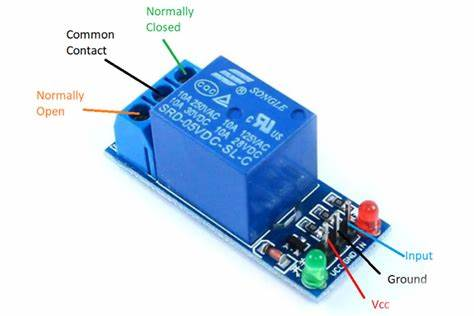
\includegraphics[width=1.0\linewidth, height = 5cm]{Relay Module.jpg} 
\caption{Relay Module}
\label{fig:Relay Module}
\end{wrapfigure}

Micro-Controller can pass voltage only upto 5V level, so we need a device which can connect to the \uline{'AC Lines'}.\\

Relays are the link between the \uline{Low-powered digital electronics} and the \uline{High-powered devices}.

Relays allow digital circuits and digital micro-controllers to switch high powered devices ON and OFF. These are simple switches which can be activated by taking pulse from micro-conntroller.\\

In this Project, \uline{3 Relays} are used (for Mainroom's Bulb, Washroom's Bulb, and for a Bulb which is used as Prototype for Cooling system). From the image we can see the pin-out configuration of the Relay module. 

The input of 230V AC is given to \uline{\textit{Relay Common (COM) pin}}. The load is connected to the \uline{\textit{Normally Open (NO)}} pin of the Relay. Initially Relay 'COM' pin and \uline{\textit{Normally Closed (NC) pin}} is \uline{shorted}.\\

When the output of PIC16F887 goes HIGH, then the corresponding Relay is switched ON, and 'COM' pin is connected to 'NO' pin of the Relay, turning ON the load. 

If the output of the Controller is LOW, then the corresponding Relay is switch OFF, and 'COM' pin is shorted with 'NC' pin of the Relay, turning OFF the load.

\subsection{DS3231 RTC Module:}

\begin{wrapfigure}{R!htbp}{0.4\textwidth}	%Wrapping Text around a figure
\centering
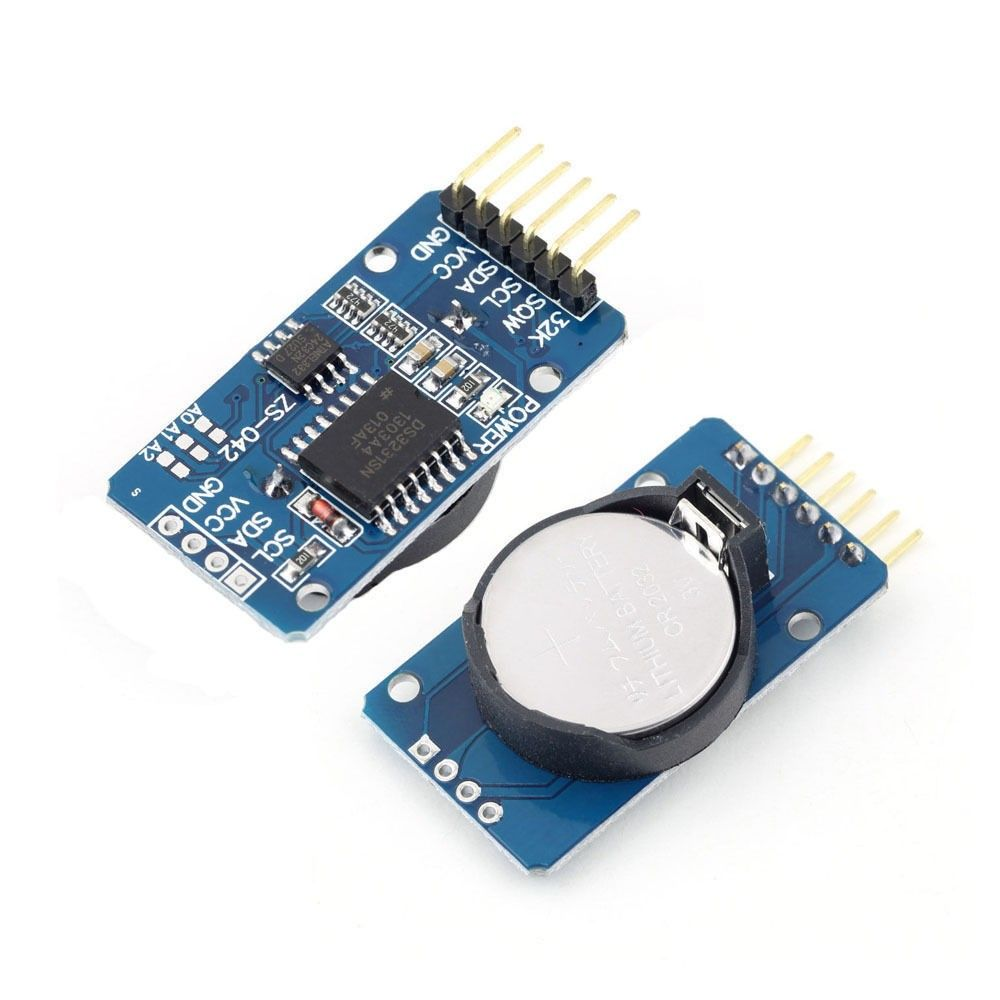
\includegraphics[width=1.0\linewidth, height = 5cm]{DS3231.jpg} 
\caption{DS3231 RTC Module}
\label{fig:DS3231 RTC Module}
\end{wrapfigure}

With the help of \uline{RTC, Real Time Clock Module}, we can give exact time of the real world to the Micro-Controller and execute according to it. DS3231 is a low-cost, extrememly accurate I2C real-time clock/calender with an integrated Temperature compensating 32KHz Oscillator.\\ 

There are particular Registers for the \textit{Time, Calender, Alarms, etc.}, in this chipset and are connected on the \uline{I2C, Inter-Integrated Circuit Bus line}.
There's a \uline{Battery} (Coin cell), and a \uline{Oscillator} which works at 32KHz range are connected with this IC. \uline{32KHz Oscillator generates 1 second of Time period}.\\

We give/write time to the chip using \uline{I2C Protocol}, thereafter with the help of crystal and battery connected to the chip, the time will keep running in the chip. Hence, even if the power is lost and Controller stops executing, it will always get the latest real time from the RTC chip and execute without any time delay after the power is back.\\

\subsubsection{Battery Backup:}

\begin{itemize}
\item The module is supplied with a \uline{\textit{Non-Rechargable CR2032 Li-Battery}} for maintaining accurate timekeeping when the main power to the device is interrupted.

\item From the specifications, it has been calculated that, without an external power supply, the battery can keep RTC Chip running for a \uline{minimum of 8 years (8.37 years to be precise)}.

\item It is important to note that, fresh batteries should be installed if the module is to be relied on for more than 12 months.
\end{itemize} 

\subsubsection{Features and benefits of DS3231:}

\begin{itemize}
\item The chip has a Time-keeping Accuracy of $\pm{0.452}$ sec/day and from -45\si{\degree} to +85\si{\degree}.

\item Digital Temperature Sensor with $\pm{3}$\si{\degree} accuracy.

\item Two Time-of-Day Alarms.

\item Has fast I2C Interface (400KHz).

\item When the device is powered by VCC, the time adjustment occurs 'once a second', when powered by BATTERY, the time adjustment occurs 'once in 10 seconds' to conserve power.  

\item The default \uline{Device Address is 0x68 in Decimal (D0h in Hexa-Decimal or 0b1101000 in Binary)}. The pads located to the lower right, "\uline{A0, A1, and A2}" are used to change the last 3 bits of the device's address. Shorting the pads will reduce the address down allowing upto "\uline{8 Memory Chips}" to the same I2C Bus (0b1101000 to 0b1101111).

\end{itemize}

\subsubsection{Digital Clock Application:}

With the help of DS3231 RTC Module, I've implemented the "\uline{\textit{Digital Clock}}" in this project. Programming for this is done based on the concept of \uline{\textit{FSM, Finite State Machine}}, where the state will change based on the input given by the user with the help of \textit{Switch Buttons}. The outputs of this FSM are given to \uline{LCD}. Hence, we can see/set the time and calender with the help of DS3231 RTC Chip, LCD, and Switch Buttons. 

We have mainly four Interfaces in this Digital Clock which can be seen in LCD:

\begin{enumerate}
\item \textbf{Main Interface -} In this Interface, we can see the values of Time (in AM/PM), Date, Day, Month, Year, Temperature, and check whether the communication used for operating electrical appliances is whether Bluetooth or WiFi.

\item \textbf{Menu Interface -} In this Interface, we can select the options to set Time or Day/Date.

\item \textbf{Set Time Interface -} In this Interface, we can set Hours, Minutes, and AM or PM mode.

\item \textbf{Set Date/Day Interface -} In this Interface, we can set Date, Day, Month, and Year.
\end{enumerate}

\begin{figure}[!htbp]
  \begin{subfigure}[b]{0.6\textwidth}
    \includegraphics[width=\textwidth, height=4cm]{Main Interface.jpg}
    \caption{Main Interface of Digital Clock}
    \label{fig:Main Interface of Digital Clock}
  \end{subfigure}
  \hfill
  \begin{subfigure}[b]{0.3\textwidth}
    \includegraphics[width=\textwidth, height=4cm]{Set Time.jpg}
    \caption{Menu Interface - Set Time}
    \label{fig:Menu Interface - Set Time}
  \end{subfigure}
  \hfill
  \begin{subfigure}[b]{0.3\textwidth}
    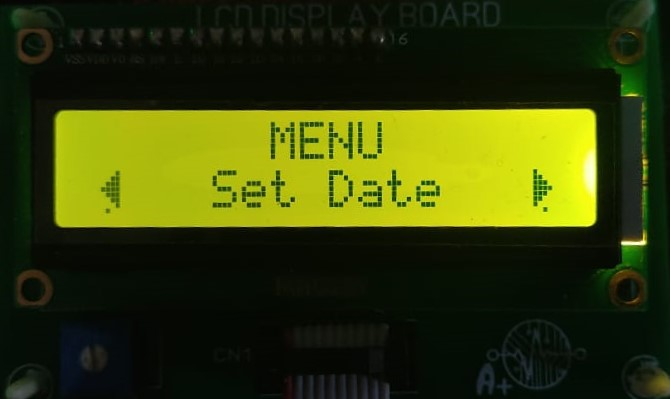
\includegraphics[width=\textwidth, height=4cm]{Set Date.jpg}
    \caption{Menu Interface - Set Date}
    \label{fig:Menu Interface - Set Date}
  \end{subfigure}
  \hfill
  \begin{subfigure}[b]{0.3\textwidth}
    \includegraphics[width=\textwidth, height=4cm]{Time Setup.jpg}
    \caption{Time Setup Interface}
    \label{fig:Time Setup Interface}
  \end{subfigure}
  \hfill
  \begin{subfigure}[b]{0.3\textwidth}
    \includegraphics[width=\textwidth, height=4cm]{Date Setup.jpg}
    \caption{Date Setup Interface}
    \label{fig:Date Setup Interface}
  \end{subfigure}
  \caption{Digital Clock}
\end{figure}



Three Buttons are used for this:
\begin{enumerate}
\item \textbf{Mode Button -} When user presses on this button, user can go the 'Menu interface' from the 'Main interface' Screen and vice-versa. And note that, this button should be pressed after setting the Date/Day or Time values in their respective interfaces to get back to the 'Main Interface'.

\item \textbf{Next Button -} When user presses on this button, user can set the values of Time, Date/Day by incrementing them. User can even long press on this button and set the values quickly.

\item \textbf{Select Button -} When user presses on this button, user can select the Time/ Date/ Day/ Month/ etc., in their respective interfaces and set the values. And user can select the options in 'Menu Interface' (i.e, "Set Time" and "Set Date/Day").
\end{enumerate}


\subsection{16x2 LCD Module:}

\begin{wrapfigure}{R!htbp}{0.4\textwidth}	%Wrapping Text around a figure
\centering
\includegraphics[width=1.0\linewidth, height = 5cm]{LCD Pinout.png} 
\caption{16x2 LCD Module Pin-out}
\label{fig:16x2 LCD Module Pin-out}
\end{wrapfigure}

As mentioned in 2.7.2 section, this LCD module is used for displaying the Digital Clock. The 16×2 LCD display is a very basic module commonly used in DIYs and circuits. The 16×2 translates to a display 16 characters per line in 2 such lines. In this LCD each character is displayed in a \uline{5×7 pixel matrix}.\\

It has an inbuilt \uline{Hitachi- HD44780 micro-controller and 128 bytes of RAM}, which takes the task of refreshing the controller and setting it with PIC16F887 micro-controller.

This module contains \uline{alpha-numeric displays from 8 to 80 characters}.
\newpage

\section{Voice IoT System:}

\begin{figure}[!htbp]
  \includegraphics[width=\linewidth, height = 7.5cm]{Voice IoT System.png}
  \caption{Voice IoT System}
  \label{fig:Voice IoT System}
\end{figure}

There are certain terminologies to understand:

\begin{itemize}
\item \textbf{Household Commissioning -} It refers to the grouping of devices (Lights, Fans, Refrigerators, etc.) and interfaces that are mutually authenticated.

\item \textbf{Voice Interface -} It is Customer premise equipment. For example, \textit{Alexa, Google Assistant, Siri}, etc. It locally listens to a trigger. To trigger it, a \uline{Wake-word} is used, like \textit{OK Google, Alexa!!, Hey Siri}, etc., before passing the voice command. It passes and listens the responses to and from the '\uline{Voice Cloud}'.

\item \textbf{Voice Cloud -} It is a Cloud based End-Point to which a voice interface connects to. It is \uline{\textit{Pre-Determined}} (Not any device can be connected, proper provisioning is required).

\item \textbf{Device Interface -} It is a \uline{Device Cloud provided mechanism} (see section 2.2.2) . It is used to control and manage the devices in device cloud. It is used by entities like Voice Cloud and Smart-phone apps to control the device. 
\end{itemize}

Figure 11 shows the overview of Voice IoT System. It can be depicted as, If a user gives a command using Google Assistant, then this Voice Command is passed to the \uline{Google Assistant Back-end}. From there, if the user gets authenticated, then the command is passed on to the Device Cloud (Adafruit Server). And finally the user command will get initiated.
\newpage

\begin{figure}[!htbp]
  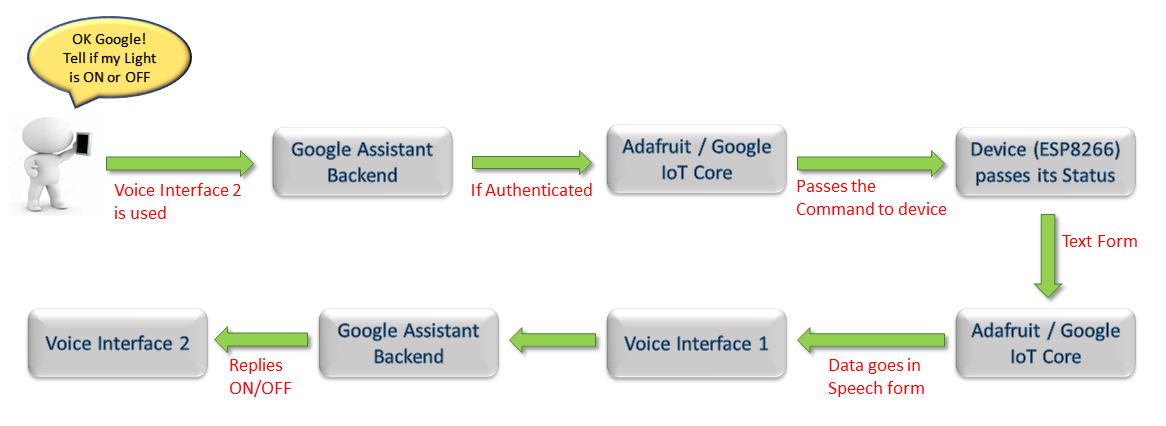
\includegraphics[width=\linewidth]{Other case of Voice IoT.png}
  \caption{Flow of Voice IoT system if user asks certain info}
  \label{fig:Flow of Voice IoT system if user asks certain info}
\end{figure}

Now, if a user wants to know the status of some device, he will ask the Voice Interface (Alexa or Google or Siri, etc) and expect some response from it. The Response flow of this case is depicted in the Figure 12.

\subsection{IFTTT Platform:}

\begin{wrapfigure}{R!htbp}{0.4\textwidth}	%Wrapping Text around a figure
\centering
\includegraphics[width=1.0\linewidth, height = 4cm]{Create Applet.jpeg} 
\caption{Create Applet Interface}
\label{fig:Create Applet Interface}
\end{wrapfigure}

IFTTT, \uline{If This Then That}, is a service that allows a user to program a response to events of various kinds. There is a long list of kinds of events to which IFTTT can respond, all detectable via the Internet.  

All we have to do is create \uline{\textit{Applets}}, which are the simple programs in IFTTT to give response to events. The interface for it looks like the Figure 13.\\

Steps involving in creating Applet are:

\begin{enumerate}
\item We have to Click on Add button of \textbf{If This}, then select a \uline{Trigger service} (Google Assistant as per this project) and select a trigger.

\item After selecting the Trigger, a new interface will appear which looks like Figure 14(b), now complete the trigger fields by filling it with what you want to say in different ways.

\item Then Click on Add button of \textbf{Then That}, and select a \uline{Action service} (Adafruit Cloud platform as per this project).

\item A new interface will appear which looks like Figure 14(c), complete the action fields and we're done.
\end{enumerate}

After successfully creating the applets, the main interface of your IFTTT account looks like Figure 14(a). Whenever you say your wake-word "OK Google" and give a command, you will get the response that you filled out in the trigger fields.\\

\begin{figure}[!htbp]
  \begin{subfigure}[b]{0.3\textwidth}
    \includegraphics[width=\textwidth]{IFTTT Interface.jpeg}
    \caption{IFTTT Main Interface}
    \label{fig:IFTTT Main Interface}
  \end{subfigure}
  \hfill
  \begin{subfigure}[b]{0.3\textwidth}
    \includegraphics[width=\textwidth]{Edit If This.jpeg}
    \caption{Complete Trigger Fields}
    \label{fig:Complete Trigger Fields}
  \end{subfigure}
  \hfill
  \begin{subfigure}[b]{0.3\textwidth}
    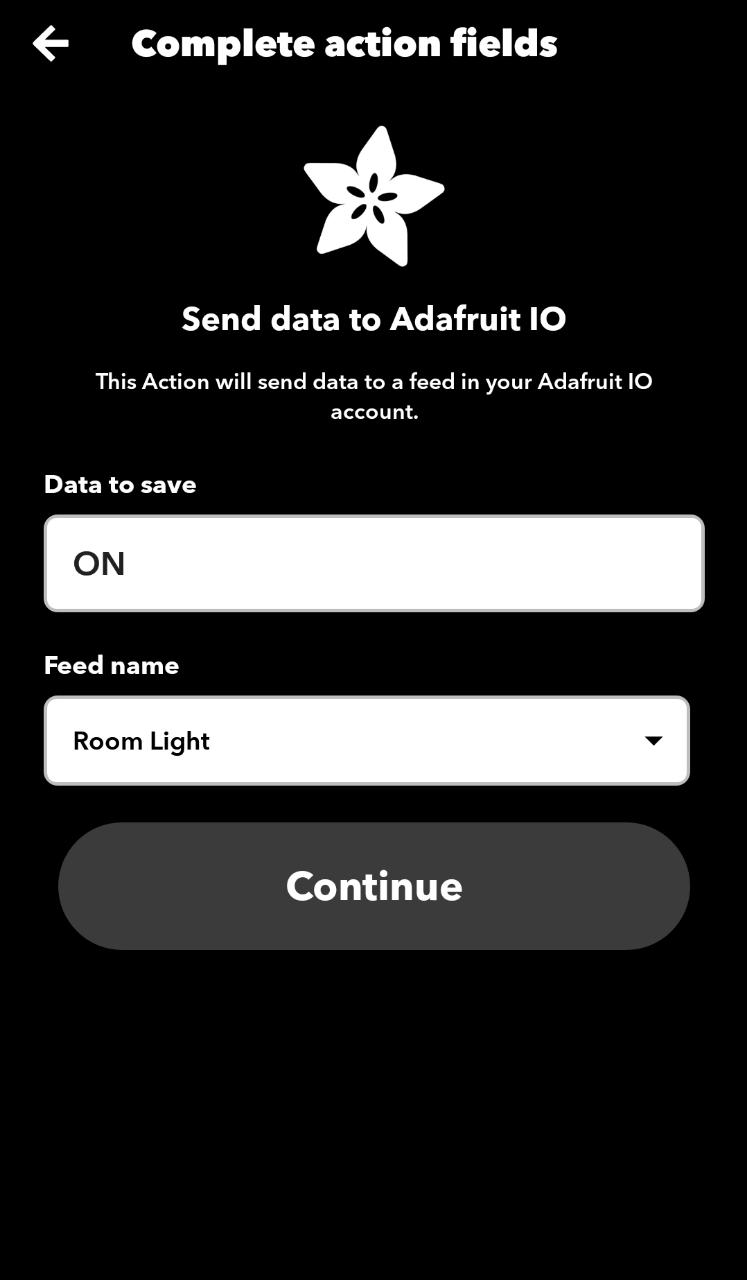
\includegraphics[width=\textwidth]{Edit Then That.jpeg}
    \caption{Complete Action Fields}
    \label{fig:Complete Action Fields}
  \end{subfigure}
  \caption{IFTTT}
\end{figure}

In this project, I have used IFTTT platform to take the trigger from 'Google Assistant' and give a response to the 'Adafruit Server' for operating Main-room's Appliances (Light and Cooling System).

\subsection{Adafruit IO:}

As depicted in section 2.2.2, Adafruit is a device cloud platform which takes the status from ESP8266 Device or commands from the user (Google Assistant).

I've created a \textit{Dashboard} named "\uline{Voice IoT Devices}". And added two feeds named \textit{Room Light}, and \textit{Cooling System} which can be seen in Figure 15(c). The interface for operating these feeds are positioned in the Dashboard and looks like Figure 15(a).\\

Whenever we use Google Assistant or Adafruit web to turn ON/OFF the Main-room Light or Cooling System, then we can see the record of all the data (when the device is operated) in feeds window of Adafruit IO, which looks like Figure 15(b). 

\begin{figure}[!htbp]
  \begin{subfigure}[b]{0.3\textwidth}
    \includegraphics[width=\textwidth, height=6.5cm]{Dashboard.jpeg}
    \caption{Adafruit IO Dashboard}
    \label{fig:Adafruit IO Dashboard}
  \end{subfigure}
  \hfill
  \begin{subfigure}[b]{0.3\textwidth}
    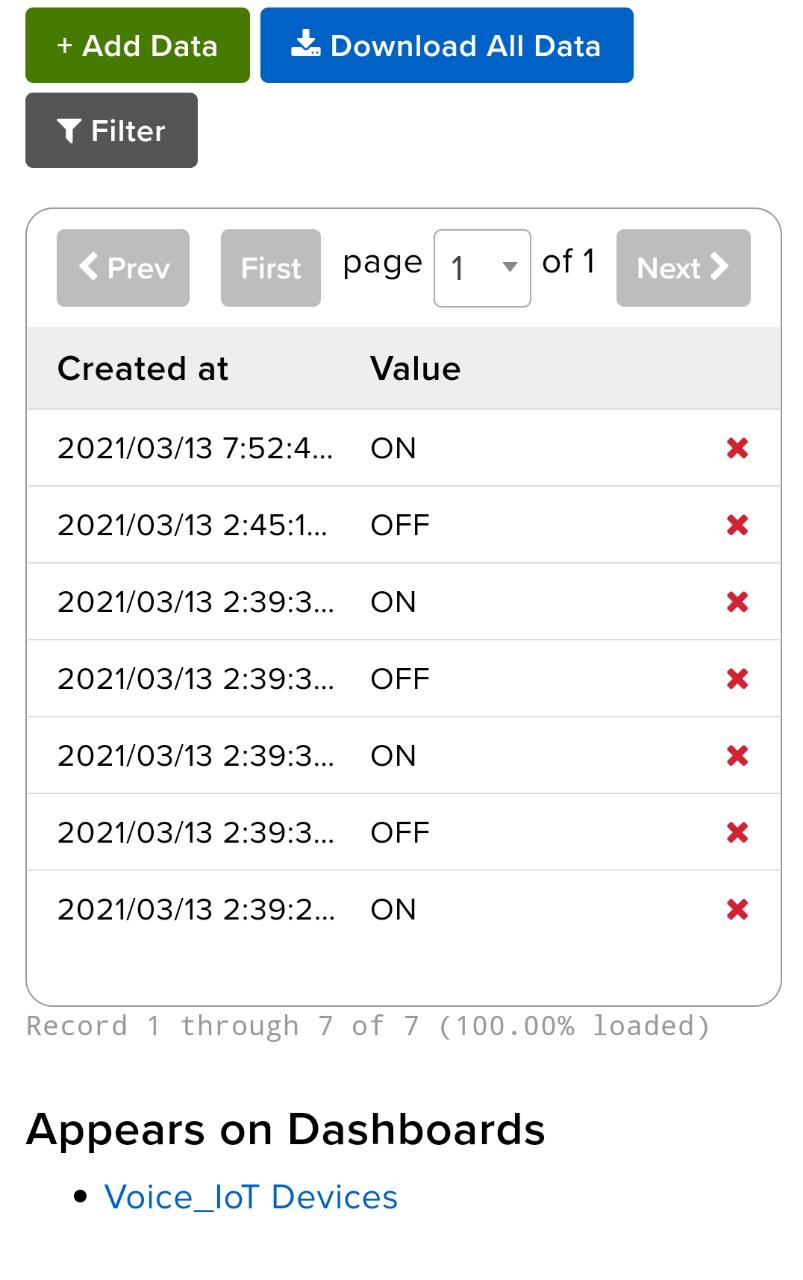
\includegraphics[width=\textwidth, height=6.5cm]{Feed Record.jpeg}
    \caption{Room Light Feed Record}
    \label{fig:Room Light Feed Record}
  \end{subfigure}
  \hfill
  \begin{subfigure}[b]{0.3\textwidth}
    \includegraphics[width=\textwidth]{Feeds.jpeg}
    \caption{Adafruit IO Feeds}
    \label{fig:Adafruit IO Feeds}
  \end{subfigure}
  \caption{Adafruit IO}
\end{figure}
 
\section{Pulse Width Modulation:}

Pulse Width Modulation or PWM is a technique for getting Analog results with Digital means. It is effective in adjusting the brightness of LEDs, or controlling speed, phase, Frequency, etc. PWM manages the Output Pulse. (If we can ON-OFF the LEDs within the intervals of few micro-seconds, then brightness can be controlled)\\

In this project, I have implemented PWM of PIC16F887 Micro-Controller for controlling \textit{Air conditioning/ Cooling System} and \textit{Washroom Bulb}. By using \uline{CCP (Capture, Compare, PWM}) and \uline{Timer2} Modules of PIC16F887, we can control the Duty Cycle for which we wish to keep the output in HIGH state.\\

\begin{itemize}
\item For the \textit{Washroom Bulb}, PWM is used in such a way that when a person enters the washroom in between 12:00 AM to 6:00 AM, brightness of the Bulb gets reduced by $60\%$ automatically so that user won't get uncomfortable when entering washroom after mid-night by facing the light.

\item And for the \textit{Cooling System}, by using formula of \uline{System of Linear Equations} and method of \uline{Common Differences}, I've made an equation such that if Temperature is 35, then Light will be turned ON with full brightness (Prototype for Cooling System) and if Temperature is around 20, then Light's Brightness will get reduced by $90\%$, and if the Temperature gradually decreases from 35 to 20 then Brightness will reduce in a systematic manner based on the equation, which indicates that cooling decreases as Temperature decreases.
\end{itemize}



\newpage

\section{Flow Charts:}
\subsection{Main-room Door IR Interfacing:}

\begin{figure}[!htbp]
  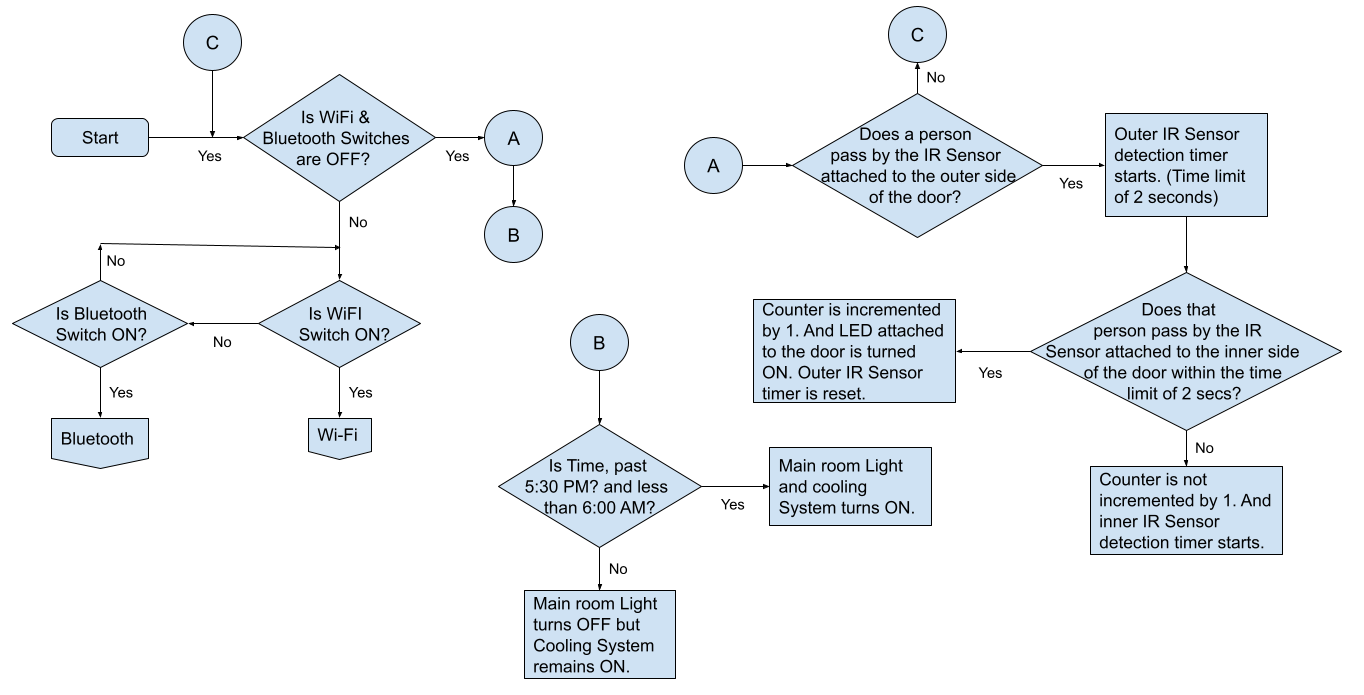
\includegraphics[width=\linewidth, height=9.2cm]{Flow Chart for the case when person enters the Main-room.png}
  \caption{Flow Chart for the case when person enters the Main-room and increment of Counter}
  \label{fig:Flow Chart for the case when person enters the Main-room and increment of Counter}
\end{figure}

\begin{figure}[!htbp]
  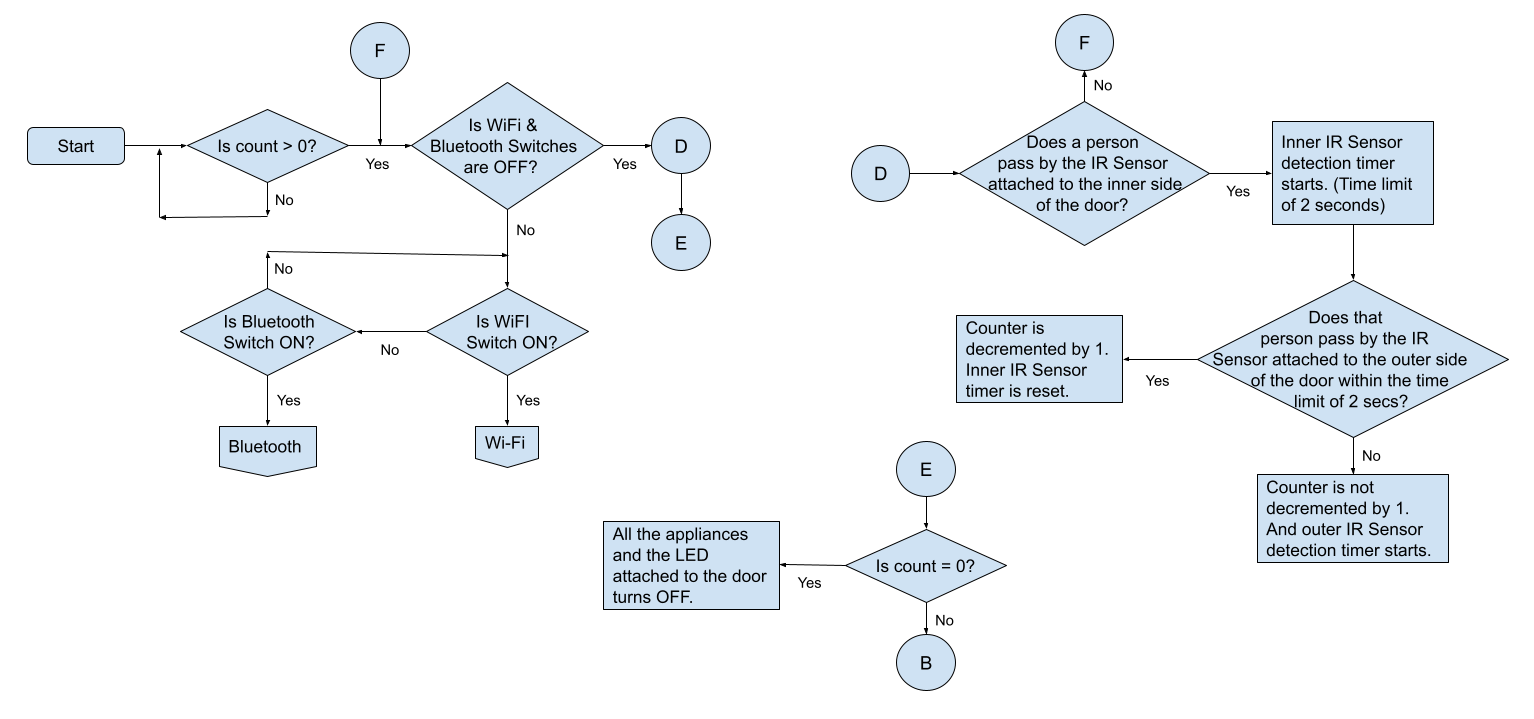
\includegraphics[width=\linewidth, height=9.2cm]{Flow Chart for the case when a person exits the Main room.png}
  \caption{Flow Chart for the case when person exits the Main-room and decrement of Counter}
  \label{fig:Flow Chart for the case when person exits the Main-room and decrement of Counter}
\end{figure}

\subsection{Washroom door IR \& PIR Interfacing:}

\begin{figure}[!htbp]
  \includegraphics[width=\linewidth, height=15cm]{Washroom Flowchart.png}
  \caption{Flow Chart for the operation of Washroom's Bulb}
  \label{fig:Flow Chart for the operation of Washroom's Bulb}
\end{figure}

\newpage
\subsection{WiFi Communication:}

\begin{figure}[!htbp]
  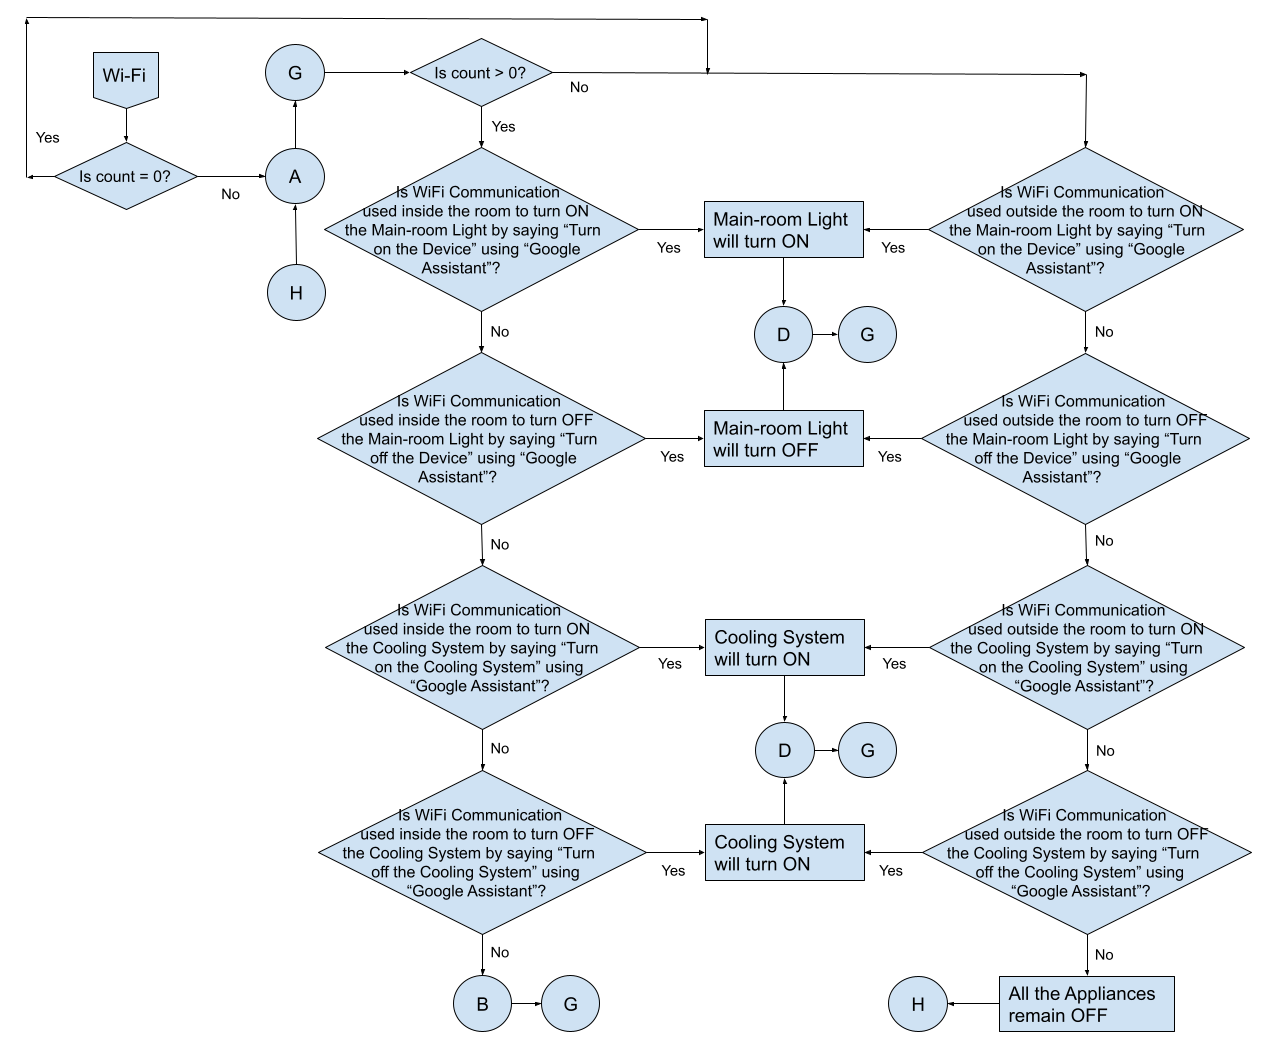
\includegraphics[width=\linewidth, height=18cm]{WiFi Communication.png}
  \caption{Flow Chart for the operation of Appliances using WiFi Communication}
  \label{fig:Flow Chart for the operation of Appliances using WiFi Communication}
\end{figure}

\newpage
\subsection{Bluetooth Communication:}

\begin{figure}[!htbp]
  \includegraphics[width=\linewidth, height=18cm]{Bluetooth Communication.png}
  \caption{Flow Chart for the operation of Appliances using Bluetooth Communication}
  \label{fig:Flow Chart for the operation of Appliances using Bluetooth Communication}
\end{figure}

\newpage
\subsection{Digital Clock:}

\begin{figure}[!htbp]
  \includegraphics[width=\linewidth, height=22cm]{Digital Clock.png}
\end{figure}

\begin{figure}[!htbp]
  \includegraphics[width=\linewidth, height=23cm]{Digital Clock 2.png}
  \caption{Flow Chart for the Digital Clock Application}
  \label{fig:Flow Chart for the Digital Clock Application}
\end{figure}

\section{Schematic Model:}

\begin{figure}[!htbp]
  \includegraphics[width=\linewidth, height=12cm]{Schematic 1.png}
\end{figure}

\begin{figure}[!htbp]
  \includegraphics[width=\linewidth, height=9cm]{Schematic 2.png}
  \caption{Schematic Model of the IoT Room Automation System}
  \label{fig:Schematic Model of the IoT Room Automation System}
\end{figure}

\section{Results:}

\begin{figure}[!htbp]
  \includegraphics[width=\linewidth, height=11.2cm]{Final Setup.jpg}
  \caption{Project Final Setup}
  \label{fig:Project Final Setup}
\end{figure}

\begin{figure}[!htbp]
  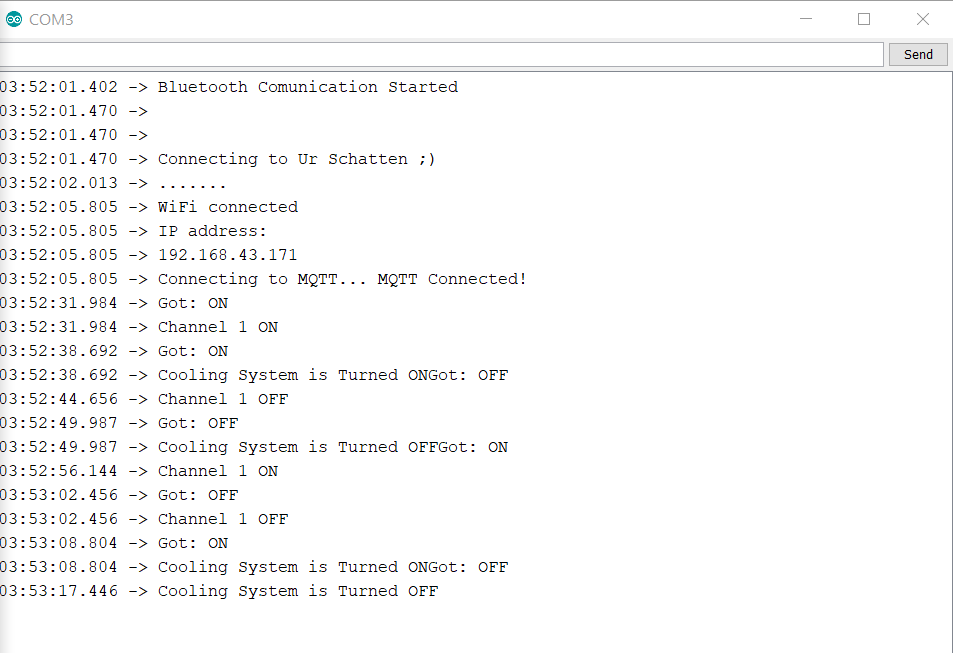
\includegraphics[width=\linewidth, height=8.7cm]{Arduino Serial Monitor.png}
  \caption{Arduino Serial Monitor}
  \label{fig:Arduino Serial Monitor}
\end{figure}

\newpage
\section{Future Scope:}

The basic vision of the system is to provide a Home Automation System using IR \& PIR Sensors for convenient secure system and connecting the whole system to the internet to make it smart, efficient, and time saving to the user, which would also aid the high degree of mobility control we aim to achieve nowadays.

Using this system as a framework, the system can be expanded to include various other options which could include:
\begin{itemize}
\item Integration of many high powered electrical appliances for operating remotely over WiFi or Bluetooth.

\item Charging the Phone for a particular time so that user can sit back and relax without worrying.

\item Adding Alarm functionality to the Digital Clock.

\item Automatic Door Lock \& unlock with the help of \textit{GPS tracking System}, so that based on my mobile's location, my home system will identify that I'm near home and automatically unlocks the door and turns ON cooling system or other appliances if necessary.

\item Home security feature like capturing the photo of a person moving around the house and storing it in the cloud., and many more modules with various other functions can be
developed and used to make a great ecosystem.
\end{itemize}

Since I've been using the free version of XC8 Compiler for MPLAB X IDE, while compiling the source code,  the \uline{Program space} of PIC16F887 is getting fully used up, therefore I couldn't integrate other features in this project. In the future, this project can be implemented with integration of many other modules on other PIC Micro-Controller series like \uline{PIC18F} series which provides sufficient program space and many inbuilt modules to make use of. 

And ESP8266 Micro-Controller is used only for WiFi/IoT Applications and Bluetooth Communication. Hence it can also be used to integrate additional features in the future to this intelligent Home System.\\

Also, with the integration of \textit{Raspberry Pi} or \textit{FPGA Processors}, \uline{Machine Learning/ Artificial Intelligence} can be implemented on the system, since if we have AI platform through which all of this is managed \& maintained, then the personalization and the human touch also comes into the picture. 

And if this AI is interconnected with IoT platform, then all the security present on each of these things gets multiplied and this will become much more secure system, since security is very essential in IoT systems (so that no third-person can actually try and manipulate our system functions for their requirements).

\section{Conclusion:}

The implementation of the system was a success and is robust enough to be used on a 24x7 basis with various normal domestic loads with very few errors (in case of counting the number of people entered or exited the room, which is depicted in section 2.4.2).\\

Main motive of this project is to have a centralized control system to operate the appliances
through a Android phone. And the model for this Room Automation System based on the idea of the Internet of Things (IoT) technology has been successfully implemented. The whole system is energy efficient, safer, secured, Time saving, flexible, and effortless.\\ 

Users can monitor and control their home appliances from anywhere around the world using cellular phone through Wi-Fi communication technology. And using Bluetooth communication, users can operate their appliances with ease in their home. 

Hence this system gives a better human interaction with things and providing better utilization of Android Phones and Micro-Controllers.\\

\end{document}
